% Created 2020-11-03 二 22:40
% Intended LaTeX compiler: xelatex
\documentclass[11pt]{report}
\usepackage{graphicx}
\usepackage{grffile}
\usepackage{longtable}
\usepackage{wrapfig}
\usepackage{rotating}
\usepackage[normalem]{ulem}
\usepackage{amsmath}
\usepackage{textcomp}
\usepackage{amssymb}
\usepackage{capt-of}
\usepackage{hyperref}
\author{曹嘉祺 PB18030874 化学与材料科学学院 有机化学系 \thanks{中国 安徽合肥 中国科学技术大学 Email: \href{mailto:mkq@mail.ustc.edu.cn}{mkq@mail.ustc.edu.cn}}}
\usepackage[scheme=plain]{ctex}
\usepackage{fontspec}
\setmainfont{更纱黑体 UI SC}
\hypersetup{colorlinks=true,linkcolor=blue}
\usepackage{longtable}
\date{\today}
\title{稀溶液粘度法测定聚合物的分子量}
\hypersetup{
 pdfauthor={曹嘉祺 PB18030874 化学与材料科学学院 有机化学系},
 pdftitle={稀溶液粘度法测定聚合物的分子量},
 pdfkeywords={},
 pdfsubject={},
 pdfcreator={Emacs 27.1 (Org mode 9.4)}, 
 pdflang={English}}
\begin{document}

\maketitle
\tableofcontents

\begin{abstract}
本文介绍了利用稀溶液粘度法测定聚合物粘均分子量的方法。利用乌氏粘度计
测定相同量的不同浓度稀溶液通过毛细管的时间,可以测定出不同浓度溶液的相对
粘度以及增比粘度,根据粘度和浓度的经验关系,可外推得到溶液的特性粘数。特
性粘数只与分子量相关,进而可由经验公式求算出聚合物的分子量。

\noindent\rule{\textwidth}{0.5pt}
\begin{itemize}
\item 关键词: 稀溶液\quad 粘度法\quad 聚乙二醇\quad 粘均分子量
\end{itemize}
\end{abstract}




\begin{abstract}


In this experiment, we learn the knowledge of average molecular weighs of polymer and
the physical meaning of viscosity average molecular weighs. What is more we know the principle of dilute
solution viscometry to determine the viscosity average molecular weighs of polymer. And we use
Ukrainian-style viscometer to determine the flow time of polyethylene glycol of different concentration,
then by calculation, we can get the average molecular weighs of polyethylene glycol.



\noindent\rule{\textwidth}{0.5pt}

\begin{itemize}
\item key words:  Viscosity-average molecular weight, viscosity, dilute solution viscometry, relative, viscosity, specific viscosity, intrinsic viscosity, Ukrainian-style viscometer, polyethylene glycol
\end{itemize}
\end{abstract}
\part{前言}
\label{sec:orgc07c2bc}
  液体的流动是因受外力作用分子进行不可逆位移的过程。液体分子间存在着相互作
用力,因此当液体流动时,分子间就产生反抗其相对位移的摩擦力(内摩擦力),液体
的粘度就是液体分子间这种内摩擦力的表现。
稀溶液粘度法测定聚合物的分子量不是一种测定分子量的绝对方法,而是一种相对
方法,因为特性粘数-分子量经验关系式是要用分子量绝对测定方法来校正订定的,本
方法也就适用于各种分子量范围。在不同分子量范围里,可能要用不同的经验方程式。
液体粘度的绝对值测定是很困难的,所以一般应用都测定相对粘度。在用稀溶液粘度法
表征高聚物分子量时,也只要测定不同浓度稀溶液的相对粘度。
\chapter{分子量的统计平均意义}
\label{sec:org42d7487}
   测定聚合物分子量的方法很多。 各种方法都有它的优缺点和适用的分子量范围, 由不同
方法得到的分子量的统计平均意义也不一样,如下表:
\begin{center}
\begin{tabular}{lll}
测定方法 & 适用的分子量范围 & 平均分子量\\
\hline
端基分析法 & <3\texttimes{} 10\textsuperscript{4} & 数均分子量\\
沸点升高法 & <3\texttimes{} 10\textsuperscript{4} & 数均分子量\\
冰点降低法 & <3\texttimes{} 10\textsuperscript{4} & 数均分子量\\
气相渗透压法 & <3\texttimes{} 10\textsuperscript{4} & 数均分子量\\
膜平衡渗透压法 & 5\texttimes{} 10\textsuperscript{3} \textasciitilde{} 10\textsuperscript{6} & 数均分子量\\
电子显微镜法 & >5\texttimes{} 10\textsuperscript{5} & 数均分子量\\
光散射法 & >10\textsuperscript{2} & 重均分子量\\
稀溶液粘度法 & >10\textsuperscript{2} & 粘均分子量\\
体积排斥色谱法 & >10\textsuperscript{2} & 各种平均分子量\\
\end{tabular}
\end{center}
\chapter{液体粘度、特性粘数及测量原理}
\label{sec:orgd1b7e75}
   采用稀溶液粘度法测定聚合物的分子量,所用仪器设备简单,操作便利,适用的分子量
范围大, 又有相当好的实验精确度, 因此粘度法是一种目前广泛应用的测定聚合物分子量的
方法。但它不是一种测定分子量的绝对方法,而是一
种相对方法,因为特性粘数-分子量经验关系式是要
用分子量绝对测定方法来校正订定的,本方法也就适
用于各种分子量范围。需注意的是在不同分子量范围
里,可能要用不同的经验方程式。
\begin{center}
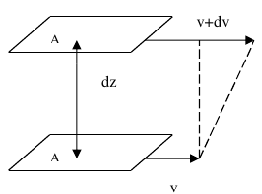
\includegraphics[width=200]{../img/1.png}
\end{center}
液体的流动是因受外力作用分子进行不可逆位移
的过程。液体分子间存在着相互作用力,因此当液体
流动时,分子间就产生反抗其相对位移的摩擦力(内
摩擦力),液体的粘度就是液体分子间这种内摩擦力的表现。
依照 Newton 的粘性流动定律,当两层流动液体面间(设面积为 A)由于液体分子间的
内摩擦产生流速梯度\(\frac{\delta v}{\delta z}\) 时
 ,液体对流动的粘性阻力是:
 \[
 f=A\eta \frac{\delta v}{\delta z}
 \]
\(\eta\) 就是液体的粘度,单位是帕斯卡\(\cdot\) 秒。
\begin{center}
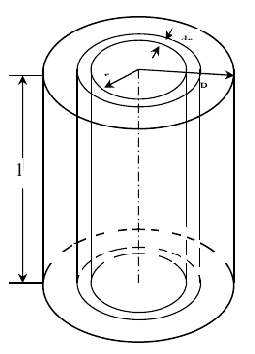
\includegraphics[width=170]{../img/2.png}
\end{center}
当液体在半径为 R 、长度为 L 的毛细管里流动时 
 ,如果在毛细管两端间的压力差为 P ,并且假使促进液
体流动的力(\(\pi\) R\textsuperscript{2}P)全部用以克服液体对流动的粘性阻
力。那么在离轴 r 和(r+dr)的两圆柱面间的流动服从
下列方程式:
\[
\pi r^{2}P+2\pi rL\eta \frac{d v}{d r}=0
\]

上式 就规定了液体在毛细管里流动时的流速分布 v(r) 。
假如液体可以润湿管壁,管壁与液体间没有滑动,则
v(R)=0 ,那么:
\[
v(r)=\int^{r}_{R} \frac{d v}{d r}d r=-\frac{P}{2L\eta}\int^{r}_{R}r dr=\frac{P}{4L\eta}\left(R^{2}-r^{2}\right)
\]
所以平均流出容速(设在 t 秒内流出液体的体积是 V)是:
\[
\frac{V}{t}=\int^{R}_{0}2\pi rvdr=\frac{\pi P}{2L\eta}\int^{R}_{0}r\left(R^{2}-r^{2}\right)dr=\frac{\pi PR^{4}}{8L\eta}
\]
则液体的粘度可表示为:
\[
\eta=\frac{\pi P R^{4}}{8LV}t
\]

液体粘度的绝对值测定是很困难的, 所以一般应用都测定相对粘度。在用稀溶液粘度法
表征高聚物分子量时,也只要测定不同浓度(C)稀溶液的相对粘度。

若以\(\eta\)\textsubscript{0}表示纯溶剂的粘度,\(\eta\) 表示溶液的粘度,则溶液的相对粘度为:
\[
\eta_{r}=\frac{\eta}{\eta_{0}}
\]
高分子溶液的粘度一般都比纯溶剂的粘度要大一些,溶液粘度增加的分数为溶液的增比粘度:
\[
\eta_{sp}=\frac{\eta -\eta_{0}}{\eta_{0}}=\eta_{r}-1
\]
而\(\frac{\eta_{sp}}{C}\) 叫做比浓粘度,\(\frac{ln\eta_{r}}{C}\) 叫做比浓对数粘度,
由于\(\frac{\eta_{sp}}{C}\) 和\(\frac{ln\eta_{r}}{C}\) 都随溶液浓度改变而改变,
而极稀溶液的相对粘度测定,不易准确, 所以常用外推到C -> 0 时的\(\frac{\eta_{sp}}{C}\) 和
\(\frac{ln\eta_{r}}{C}\) 值,这里,当浓度 C 不大时:
\[
\frac{ln\eta_{r}}{C}=\frac{ln\left(1+\eta_{sp}\right)}{C}=\frac{\eta_{sp}}{C}\left(1-\frac{1}{2}\eta_{sp}+\frac{1}{3}\eta_{sp}^{2}-...\right)
\]
所以有:
\[
\lim_{C\to 0}\frac{ln\eta_{r}}{C}=\lim_{C\to 0}\frac{\eta_{sp}}{C}
\]
令:
\[
\lim_{C\to 0}\frac{ln\eta_{r}}{C}=\lim_{C\to 0}\frac{\eta_{sp}}{C}=[\eta]
\]
这个 C->0 时的外推值 [\(\eta\)] 称为高分子的特性粘数, 其单位是为
毫升/克或分升/克,与溶液浓度的单位相对应。对于给定的体系, 特性
粘数随分子量增加而增加, 因此其值可作为分子量的量度。

从溶液的比浓粘度\(\frac{\eta_{sp}}{C}\) 和比浓对数粘度\(\frac{ln\eta_{r}}{C}\) 求取高分子的特性粘数 [\(\eta\) ]
需要有适合的粘度与浓度C的依赖关系,通常
只有通过线性的外推, 才能得到可靠的外推值。表达溶液粘度的浓度依赖性的经验方程式很
多,常用如下两个经验方程式,即 Huggins 方程式:
\[
\frac{\eta_{sp}}{C}=[\eta]+k[\eta]^{2}C
\]
和 Kraemer 方程式:
\[
\frac{ln\eta_{r}}{C}=[\eta]-\beta [\eta]^{2}C
\]
两式中,k 和\(\beta\) 均为常数。
用\(\frac{\eta_{sp}}{C}\) 对C和\(\frac{ln\eta_{r}}{C}\) 对C作图,外推
到 C -> 0 所得的截距,应重合于一点,即 [\(\eta\)] 值(下图).
\begin{center}
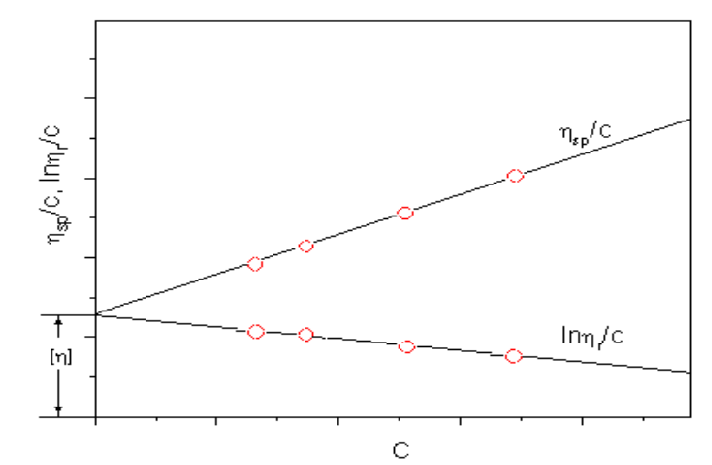
\includegraphics[width=200]{../img/3.png}
\end{center}


需要注意的是,有的溶液比浓对数粘度与浓度的关系并不呈线性,尤其在浓度较高时,
发生偏离(向下弯曲或向上弯曲)。当出现这种情况时,建议使用Huggins 方程式求取 [\(\eta\) ] 值。因为
Huggins 方程式和和 Kraemer 方程式均是通过对下式作近似处理而得到的:
\[
\frac{\eta_{sp}}{C}=\frac{[\eta]}{1-k[\eta]C}
\]
其中,k 为常数。在推导Huggins 方程式时只作了一次近似处理,而推导 Kraemer 方程式时作了两次近似
处理。具体近似处理如下:

当 k[\(\eta\)]C\(\ll\) 1时,利用一级级数展开式:
\[
\left(1-k[\eta]C\right)^{-1}=1+k[\eta]C+...
\]
略去高次项, 代入上式即得Huggins 方程式
 ,大多数高分子稀溶液的比浓粘度与浓度的关系都符合这个关系;

当\(\eta\)\textsubscript{sp} < 1时,ln\(\eta\)\textsubscript{r} 可按 Taylor 级数展开,即
\[
ln\eta_{r}=ln\left(1+\eta_{sp}\right)=\eta_{sp}-\frac{\eta_{sp}^{2}}{2}+\frac{\eta_{sp}^{3}}{3}+...
\]
把Huggins 方程式代入上式,略去高次项,得:
\[
\frac{ln\eta_{r}}{C}=[\eta]-\left(\frac{1}{2}-k\right)[\eta]^{2}C+\left(\frac{1}{3}-k\right)[\eta]^{3}C^{2}+...
\]
若 \(k=\frac{1}{3}\) ,且令\(\beta=\frac{1}{2}-k\) ,则得到Kraemer 方程式。
显然,若\(k\neq \frac{1}{3}\) ,\(\frac{ln\eta_{r}}{C}\sim C\) 的图形不再是
直线, 当浓度较高时, 曲线向下弯曲(\(k>\frac{1/3}\) ) 或向上弯曲 (\(k<\frac{1}{3}\) )
 , 曲线切线在外推到 C->0所得的截距与\(\frac{\eta_{sp}}{C}\sim C\) 作图的直线在
外推到 C->0所得的截距将不重合于一点。这时最好
使用 Huggins 方程式
 ,用\(\frac{\eta_{sp}}{C}\sim C\) 的作图的外推值求取 [\(\eta\)] 值。

\chapter{特性粘数与高分子的粘均分子量}
\label{sec:org3a243df}
当确定了高分子的特性粘数[\(\eta\)] ,就可根据特性粘数与分子量的关系式[\(\eta\)]\(\sim\) M 求取高
分子的分子量 M 。有时也直接用 [\(\eta\)] 值来表示 M 的大小。
在早期工作中, 人们就从理论上得出, 特性粘数与分子量的关系式取决于高分子在溶液
中的形态。在溶液内高分子线团如果蜷得很紧,在流动时线团内的溶剂分子随着高分子一起
流动,则高分子的特性粘数与分子量的平方根成正比,[\(\eta\)]\(\propto\) M\textsuperscript{1/2} ;假如线团松懈,在流
动时线团内的溶剂分子是完全自由的, 那么高分子的特性粘数应与分子量成正比, [\(\eta\)]\(\propto\) M 。
目前常用一个包含两个参数的 Mark-Houwink-Sakurada 经验式表示特性粘数与分子量的关
系:
\[
[\eta]=KM^{a}
\]
式中,参数 K,a 值需经测定分子量的绝对方法订定后才可使用。订定方法是,先将高聚
物按分子量分级,测定各级分的特性粘数 [\(\eta\)] 和平均分子量 M ,以 log [\(\eta\)] 对 log M 作
图,假如 a 是常数, log [\(\eta\)] \(\sim\) log M 的作图是直线,其斜率就是 a ,截距是 log K 。假如
在实验的分子量范围内, a 不是常数,那么就从 log [\(\eta\)] \(\sim\) log M 作图的曲线上求取各段分
子量范围内适用的 K 、 a 值。对于常见的聚合物溶液体系, K 、 a 值可以从有关手册或本
教材附录中查到。对于大部分高分子溶液来说, a 的数值在 0.5\(\sim\) 1.0 之间。
由于高分子的特性粘数和分子量的关系方程式 [\(\eta\)] \(\sim\) M ,视高分子在溶液里的形态而
异,而高分子的形态是高分子链段间和高分子―溶剂分子间相互作用力的反映,因此
[\(\eta\)]\(\sim\) M 关系式随所用溶剂、测定温度不同而不同。根据Flory特性粘数方程式:
\[
[\eta]=\phi \frac{\left(\bar{h^{2}}\right)^{3/2}}{M}
\]

这里 h 是高分子链的均方末端距,\(\phi\) 是一个与高分子、溶剂以及温度无
关的通用常数。在\(\theta\) 溶液中,高分子链单元间无远程相互作用,高分子尺寸恰好不受溶剂
的影响,线团处于一种无扰态,呈高斯无规线团形态,均方末端距\(\bar{h^{2}}=\bar{h_{0}^{2}}\propto M\) ,
在这种情况下, [\(\eta\)]\(\sim\) M 关系式可写成
\[
[\eta]_{\theta}=KM^{1/2}
\]
如无规聚甲基丙烯酸甲酯-乙腈溶液在45°C(\(\theta\) 温度)时,[\(\eta\)]\(\sim\) M关系式为
\([\eta]=0.048M^{0.50} (ml/g)\) ,无规聚甲基丙烯酸甲酯—氯丁烷溶液在 35.4°C(\(\theta\) 温度)时,
[\(\eta\)]\(\sim\) M关系式为 \([\eta]=0.0505M^{0.50}(ml/g)\) 。而在其它情况下,\(\bar{h^{2}}\neq \bar{h_{0}^{2}}\) ,
定义扩张因子
\[
\chi =\left(\frac{\bar{h^{2}}}{\bar{h_{0}^{2}}}\right)^{1/2}
\]
则有
\[
[\eta]=\phi \frac{\left(\bar{h_{0}^{2}}\chi^{2}\right)^{3/2}}{M}=\phi \left(\frac{\bar{h_{0}^{2}}}{M}\right)^{3/2}M^{1/2}\chi^{3}
\]
这里,\(\bar{h_{0}^{2}}/M\) 是常数,,再根据 Flory 导出的:
\[
\chi^{5}-\chi^{3}=2C_{M}\Psi_{1}(1-\theta/T)M^{1/2}
\]

可知, \(\chi\) 依赖于 M ,因此 [\(\eta\)]\(\sim\) M 关系式仍可写成\([\eta]=KM^{a}\) 的形式,其中的 a 值主要反映了\(\chi\) 对 M 的
依赖性。如无规聚甲基丙烯酸甲酯—丙酮溶液在 25°C(良溶剂条件)时, [\(\eta\)]\(\sim\) M 关系式
中 a = 0.69 > 0.50 。这里高分子线团扩张,排除体积效应较大,这是由于良溶剂分子与高
分子链单元间的相互作用克服了链单元间的吸引力(高分子间的内聚力)
 ,溶剂的作用使同
一高分子链的链单元间呈现相斥的力。而当溶剂变劣时,排斥体积则减小,线团收缩。如
25°C时无规聚甲基丙烯酸甲酯在乙腈和氯丁烷中的 a 值分别为 0.33 和 0.38,均小于 0.50。

注意:上式所表示的 [\(\eta\)] 和 M 间的函数形式,不能认为是有基础意义的,只能看作
是在一定分子量范围内,[\(\eta\)] 和 M 间联系关系的近似内插公式。在某些情况下,其它函数形
式可能更好地表达实验数据。如聚环氧乙烷—水溶液在在 25°C时, [\(\eta\)]\(\sim\) M 关系式为
[\(\eta\)] = 2.0 + 0.016M\textsuperscript{0.76} ,聚乙酸乙烯酯—丙酮溶液在在 30°C时, [\(\eta\)]\(\sim\) M 关系
式为
[\(\eta\)] = 0.097M\textsuperscript{0.50} + 0.00723M\textsuperscript{0.90} 。

\chapter{特性粘数的具体测量方法}
\label{sec:orgd507b88}
测 定 高 分 子 溶 液 的 粘 度 以
Ubbelohde 式稀释粘度计最为合适。
\begin{center}
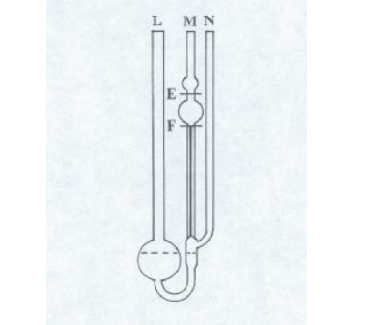
\includegraphics[width=250]{../img/4.png}
\end{center}

将液体自L管加入,在 M 管将液体
吸至E线以上后,任其流下,这样促使
流动的力,就是液柱高 h 的压力,h 值在
h\textsubscript{e} 和 h\textsubscript{f} 间逐渐改变,并且假设促使液体
流动的力全部用于克服内摩擦力, 即认为
液体在流动时没有消耗能量 (一般选择纯溶剂流出时间大于 100 秒的粘度计, 就可以略去流
动时能量损耗的主要部分——动能消耗的影响)
 。这样液体粘度即为:
\[
\eta=\frac{\pi gh\rho R^{4}t}{8LV}
\]
式中, g为重力加速度, h为流经毛细管的液柱的平均高度, \(\rho\) 为所测液体的密度, t为
液面从 a线流到 b线所需的时间(流出时间),令
\[
A=\frac{\pi ghR^{4}}{8LV}
\]
显然 A是由粘度计所决定
的常数,与液体性质无关。则高分子溶液的粘度
\[
\eta =A\rho t
\]
纯溶剂的粘度:
\[
\eta_{0}=A\rho_{0}t_{0}
\]
当测定的溶液很稀时,\(\rho \approx \rho_{0}\) ,所以:
\[
\eta_{r}=\frac{\eta}{\eta_{0}}\approx \frac{t}{t_{0}}
\]
\[
\eta_{sp}=\eta_{r}-1\approx \frac{t}{t_{0}}-1
\]
这样只要在同一温度下测定纯溶剂和不同浓度C的聚合物溶液流经 a、b 线的时间 t\textsubscript{0}和
t( t\textsubscript{1} 、 t\textsubscript{2} 、 t\textsubscript{3} 、 t\textsubscript{4} 、 t\textsubscript{5} )就可算出不同浓度溶液对溶剂的相对粘度 \(\eta\)\textsubscript{r} ,
继而计算出 \(\eta\)\textsubscript{sp} 、ln(\(\eta\)\textsubscript{r})等,
然后从\(\frac{\eta_{sp}}{C}\sim C\) 以及\(\frac{ln\eta_{r}}{C}\sim C\) 作图外推得到高分子的特性粘数 [\(\eta\)] ,
最后根据\([\eta]\sim M\) 关系式求取聚合物分子量 M 。

因为需要测定不同浓度溶液的相对粘度,最简便且适用的方法是在粘度计里逐渐稀释
(详见操作步骤)
 ,可以节省许多操作手续,故采用气承悬液柱式的稀释粘度计最为合适,
因为液体的流出时间与粘度计中液体体积无关。
本实验是在同一支粘度计内测定一系列浓度成简单比例关系的溶液的流出时间后,再测
溶剂的流出时间。这是因为考虑到高分子溶液流过毛细管后,常会有高分子吸附在毛细管管
壁,所以相当于高分子溶液流过了较细的毛细管,为了得到高分子溶液真实的相对粘度,后
测纯溶剂的流出时间,这样,纯溶剂流过的也是较细的毛细管,消除了高分子在毛细管上的
吸附对结果的影响。反之如果在测定溶液之前测定纯溶剂的流过时间,此时毛细管并未被高
分子吸附,纯溶剂将在较短的时间内流过毛细管,测定纯溶剂流过时间的毛细管状态就和之
后测定溶液流过时间时的状态不一致, 如果高分子在毛细管管壁的吸附严重时,\(\frac{\eta_{sp}}{C}\sim C\) 的
作图将是一条凹形的曲线。
然而在有些情况下高分子在毛细管管壁的吸附还会引起界面性质的改变。 如杨海洋发现
聚乙烯吡咯烷酮(PVP)-水溶液在极低浓度区的粘度行为是反常的,而这种反常行为不能简
单地被认为是由于高分子吸附在毛细管管壁上导致毛细管有效管径减小所致。 这是由于玻璃
的表面是亲水的,而PVP是两亲性高分子,因此在测定PVP水溶液流过时间时,PVP的亲水
基团将优先吸附在毛细管管壁上,其憎水基团朝外,PVP分子在毛细管管壁上的吸附会使得
毛细管表面性质发生了显著改变,这样,流体在固体表面的张力也将因此而改变,界面性质
变化也会使流体在玻璃界面处接触角产生改变进而导致流体在流动过程中因弯曲液面而产
生的附加压强发生改变, 最终影响到流体在粘度计中的流过时间。 但是通过对粘度测定方法
进行改进也可消除界面性质变化的影响。杨海洋提出, 以高分子溶液流过时间 t 对浓度作图,
外推到浓度为零时的流出时间 t\textsubscript{0}\textsuperscript{* } 代替纯溶剂的流出时间 t\textsubscript{0} 来计算相对粘度。从测量的角度
上看, t\textsubscript{0}\textsuperscript{* }可以被认为是理想条件下溶剂在粘度计中的流出时间。显然,这种方法不仅更加
省时省力、简单易行(免去了纯溶剂流过时间的测定),而且实验结果更为合理和普适。
对于多分散的聚合物,用式(13)计算所得的分子量是一种统计平均值。根据式 Mark-Houwink-Sakurada 经验式和上述的外推结论,
有:
\[
[\eta]=\lim_{C\to 0}\frac{\eta_{sp}}{C}=KM^{a}
\]
\[
\left(\eta_{sp}\right)_{C\to 0}=KCM^{a}=K\sum_{i}C_{i}M_{i}^{a}=KC\sum_{i}\left(\frac{C_{i}}{\sum_{i}C_{i}}M_{i}^{a}\right)=KC\sum_{i}\left(W_{i}M_{i}^{a}\right)
\]
而粘均分子量的定义式为:
\[
\bar{M_{\eta}}=\left(\sum_{i}W_{i}M_{i}^{a}\right)^{\frac{1}{a}}
\]

比较上两式可知, 采用稀溶液粘度法测得的是多分散聚合物的粘均分子量\(\bar{M_{\eta}}\) ,
而且其数值不仅与分子量分布有关,还与 a 值有关。


\part{实验部分}
\label{sec:orgf99b615}
\chapter{实验仪器与试剂}
\label{sec:org093d15f}
\begin{center}
\begin{tabular}{llll}
仪器 & 数目 & 仪器 & 数目\\
\hline
乌式粘度计 & 一支 & 恒温水槽 & 一套*\\
秒表 & 一块 & 5 毫升、10 毫升移液管 & 各一支\\
25 毫升、50 毫升容量瓶 & 各一个 & 2\textsuperscript{\#}或 3\textsuperscript{\#}熔砂漏斗 & 两个\\
50 毫升烧杯 & 一个 & 聚乙二醇、蒸馏水 & 适量\\
\end{tabular}
\end{center}

*包括: 电动搅拌器、继电器、水银接触温度计、调压器、加热器、50°C温度计

\chapter{实验步骤}
\label{sec:orgefbdd6b}
\section{玻璃仪器的洗涤}
\label{sec:orga090501}
先用经熔砂漏斗滤过的水洗涤粘度计,倒挂干燥后,用新鲜温热的铬酸洗液(滤过)浸
泡粘度计数小时后,再用蒸馏水(经熔砂漏斗滤过的)洗净,干燥后待用(此步骤已由老师
帮忙完成)。
其它如容量瓶、移液管、锥形瓶也需经无尘水
 (熔砂漏斗滤过的水) 洗涤、干燥后待用。
\section{高分子溶液的配置}
\label{sec:org0b7ef3e}
准确称取聚环乙二醇 0.855 克,在烧杯中用少量水(20-25 毫升)使其全部溶解(若溶
解困难可放入恒温水槽中恒温以加快溶解)
 ,移入 50 毫升容量瓶中,用水洗涤烧杯 3-4 次,
洗液一并转入容量瓶中,并稍稍摇晃作初步混匀,然后将容量瓶置于恒温水槽
(30°C\textpm{} 0.05 °C) 中恒温,用水稀释至刻度,摇匀溶液,再用熔砂漏斗将溶液滤入一只 50 毫
升的无尘干燥的磨口锥形瓶中并加上盖子,放入恒温水槽中恒温待用。盛有无尘溶剂水
(也是经熔砂漏斗过滤过的)的锥形瓶也放入恒温水槽中恒温待用。
\section{溶液流出时间的测定}
\label{sec:org6e11f5b}
在粘度计的 B、C 管上小心地接入乳胶管,用固定夹夹住粘度计的 A 管,并将粘度计
垂直放入恒温水槽,使水面浸没 a 线上方的小球,用移液管从 A 管注入 10 毫升溶液,恒温
10 分钟后,用乳胶管夹夹住 C 管上的乳胶管,在 B 管乳胶管上用吸耳球缓慢吸取溶液,待
液面升到 a 线上方的小球一半时停止抽气,先取下吸耳球 (否则毛细管中会进入气泡影响测
定),而后放开 C 管的夹子,让空气进入 D 球,使毛细管内溶液与 A 管下端的球分开,此
时液面缓慢下降,用秒表记下液面从 a 线流到 b 线的时间,重复测三次,每次所测的时间相
差不超过 0.2 秒,取其平均值,作为 t\textsubscript{1} 。

然后再移取 5 毫升溶剂注入粘度计,将它充分混合均匀(通过 B 管利用吸耳球往粘度
计中鼓泡以混合均匀),这时溶液浓度为原始溶液浓度的 2/3,再用同样方法测定 t\textsubscript{2} 。

用同样操作方法再分别加入 5、10 和 10 毫升溶剂,使溶液浓度分别为原始溶液的 1/2、
1/3 和 1/4,测定各自的流出时间 t\textsubscript{3} 、 t\textsubscript{4} 和 t\textsubscript{5} 。

\section{纯溶剂流出时间的测定}
\label{sec:org0d8f75f}
将粘度计中的溶液倒出,用无尘溶剂 (本实验中溶剂是水) 洗涤粘度计数遍,测定纯溶
剂的流出时间 t\textsubscript{0}.

\chapter{结果分析与讨论}
\label{sec:org9bc067f}
\section{仪器及实验参数记录}
\label{sec:org47afb8f}
\begin{center}
\begin{tabular}{llllll}
粘度计号 & 内径 & 溶剂 & 温度 & 聚乙二醇质量 & 浓度C\textsubscript{0}\\
\hline
null & 0.55mm & 蒸馏水 & 30°C & 1.0055g & 0.02011g/ml\\
\end{tabular}
\end{center}
\section{实验结果}
\label{sec:org07a312d}
\begin{enumerate}
\item 以记录纯溶剂流出时间为 t\textsubscript{0}
\label{sec:orga4cc60e}
\begin{enumerate}
\item 
\label{sec:orga03e1ad}

\[
\eta_{sp}/C' \sim C'
\]
拟合方程为:
\[
\frac{\eta_{sp}}{C'}=0.2912C'+0.7191
\]
由关系式:
\[
\frac{\eta_{sp}}{C'}=[\eta]C_{0}+k[\eta]^{2}C_{0}^{2}C'
\]
有特性粘数:
\[
[\eta]=\frac{A}{C_{0}}=\frac{0.7191}{0.02011}=35.76ml/g
\]
将得到的[\(\eta\)]代入到[\(\eta\)]=KM\textsuperscript{a},粘均分子量:
\[
\bar{M_{\eta}}=(35.76/0.0125)^{\frac{1}{0.78}}=27001.89
\]

\item 
\label{sec:orga52c511}
\[
ln\eta_{r}/C' \sim C'
\]
拟合出的曲线如下:
\[
\frac{ln\eta_{r}}{C'}=-0.03085C'+0.7317
\]
由关系式:
\[
\frac{ln\eta_{r}}{C'}=[\eta]C_{0}-\beta[\eta]^{2}C_{0}^{2}C'
\]
有特性粘数:
\[
[\eta]=\frac{A}{C_{0}}=\frac{0.7317}{0.02011}=36.38ml/g
\]
将得到的[\(\eta\)]代入到[\(\eta\)]=KM\textsuperscript{a},粘均分子量:
\[
\bar{M_{\eta}}=(36.38/0.0125)^{\frac{1}{0.78}}=27603.55
\]
\end{enumerate}

\item 以外推浓度为 0 的时间为 t\textsubscript{0}
\label{sec:org36f8052}
以 t 对 C'作图,结果如下:

\[
t\sim C'
\]
拟合出的曲线如下:
\[
t=116.87C'+98.64
\]
外推浓度为 0 时有
\[
t_{0}^{\*}=98.64
\]
\begin{enumerate}
\item 
\label{sec:org600e462}
\[
\eta_{sp}/C'\sim C'
\]
拟合出的曲线如下:
\[
\frac{\eta_{sp}}{C'}=-0.04697C'+1.2166
\]

由关系式:
\[
\frac{\eta_{sp}}{C'}=[\eta]C_{0}+k[\eta]^{2}C_{0}^{2}C'
\]
有特性粘数:
\[
[\eta]=\frac{A}{C_{0}}=\frac{1.2166}{0.02011}=60.50mL/g
\]
将得到的[\(\eta\)]代入到[\(\eta\)]=KM\textsuperscript{a},粘均分子量:
\[
\bar{M_{\eta}}=(60.50/0.0125)^{\frac{1}{0.78}}=52982.88
\]

\item 
\label{sec:orgdbeddd0}
\[
ln\eta_{r}/C' \sim C'
\]
拟合出的曲线如下:
\[
\frac{ln\eta_{r}}{C'}=-0.3802C'+1.1390
\]

由关系式:
\[
\frac{ln\eta_{r}}{C'}=[\eta]C_{0}-\beta[\eta]^{2}C_{0}^{2}C'
\]
有特性粘数:
\[
[\eta]=\frac{A}{C_{0}}=\frac{1.1390}{0.02011}=56.64mL/g
\]
将得到的[\(\eta\)]代入到[\(\eta\)]=KM\textsuperscript{a},粘均分子量:
\[
\bar{M_{\eta}}=(56.64/0.0125)^{\frac{1}{0.78}}=48689.80
\]
\end{enumerate}
\end{enumerate}


\section{结果讨论}
\label{sec:org4ec960b}
\begin{enumerate}
\item 
\label{sec:org2ba9fe8}
由实验结果可知,以记录纯溶剂流出时间作为 t\textsubscript{0} 时,按两公式处理所得的特性粘数[\(\eta\)]值基本是重合的,相对误差为:

\[
\frac{36.38-35.76}{36.38}=1.70\%
\]
但是以外推浓度为 0 时的流出时间作为 t\textsubscript{0} 时,两公式所得结果之间有较大差异,相对误差为:
\[
\frac{60.50-56.64}{60.50}=6.38\%
\]
拟合直线的线性也较差。
造成这种现象的原因可能是纯溶
剂的流出时间测量值偏大,导致计算所得的相对粘度\(\eta\)\textsubscript{r}偏小,同时可能使数据偏离线性,
进而使截距偏小, 最终使得粘均分子量偏小。而导致所测时间偏大的原因可能是由于毛细管
没有洗涤干净,残留有少许聚乙二醇高分子,毛细管局部变细且使溶剂水的粘度增大,最终
使得流出时间偏大。

\item 
\label{sec:org50084b6}
由结果可知两种不同处理方法所得结果的差异也较大,彼此间相对误差
接近 40\%。理论上说外推浓度为 0 得到的时间 t\textsubscript{0} 更具有普适性及实验意
义,但就实验结果而言,直接测量 t\textsubscript{0} 得到的结果线性更好也更可靠。实
际上采用外推浓度为 0 得到的时间 t\textsubscript{0} 对溶液实际浓度的依赖性较大,如
果测量时溶液混合不均匀,会对浓度项产生较大影响,从而对外推 t\textsubscript{0} 产
生较大影响。

\item 
\label{sec:org9193b5b}
实验过程中发现,浓度较大的组测量时间时差异较大,经稀释后时间的
差异明显减小,这可能是因为浓度较大时,毛细管壁吸附有较多的高分
子,吸附状况的差异会对时间产生较大影响。 (也有可能是实验开始阶段
对毛细管的润洗不够充分。
\end{enumerate}


\section{误差分析}
\label{sec:org2dccffb}
\begin{enumerate}
\item 实验中配制溶液过程中可能会有误差。
\item 从原理上实验中忽略了液体的动能,尽管该项很小,但还是会对结果有一定影响。
\item 实验原理上认为稀溶液密度与溶剂密度一致,可实际上二者是有差异的。
\item 实验过程中加水稀释时只是在粘度计内进行,而实际上高分子不是好的分散质,在粘度计内可能并不能够混合均匀。浓度项的误差会极大地影响外推浓度 0 时 t 的值,这可能也是采用该法误差较大的原因。
\item 加溶液及水的过程中会有部分残留在 A 管中且无法洗涤,会给浓度项带来误差。
\item 实验中只是开始时调节粘度计竖直,后来加水过程中也有可能造成粘度计不竖直,带来误差。
\item 实验中对时间的判断存在较大的人为误差。
\item 实验中对 B 管润洗不充分,造成毛细管内吸附状况的差异,也会影响对时间的测定。
\item 实验过程中发现,大的气泡可以排除,但是一些很细小的气泡很难避免,可能会对溶液的流动产生影响。
\end{enumerate}

\section{实验思考}
\label{sec:org9ab5168}
\begin{enumerate}
\item 本实验中是采取了一系列的近似,并且有很多的经验公式,不同经验公式之间会有一定差异,这可能也是造成结果差异的原因之一。
\item 实验中保证毛细管洁净非常重要,为保证时间的重复性,对毛细管的润洗也非常重要。
\item 查阅文献可知,除讲义中经验公式外,也可采用其他经验公式,例如:\([\eta]=[(ln\eta_{r})/c]\times \eta_{r}^{1/9}\) 等,具体算法不详述。
\end{enumerate}

\part{结论}
\label{sec:org84f9a52}
  本实验学习了粘度的知识及测量方法,并了解了高分子粘均分子量的计算方法。实验时
利用乌式粘度计测量了不同浓度的聚乙二醇高分子溶液及纯溶剂水的流出时间,并通过相关
数据处理求得溶液的相对粘度及聚乙二醇的粘均分子量,所得曲线和结果与理论符合的较
好,所以本实验基本上达到了预期目标。

\part{参考文献}
\label{sec:org86ab395}
\begin{enumerate}
\item 中国科学技术大学化学实验教学中心物理化学实验讲义
\item 《物理化学下》傅献彩等编 高等教育出版社
\item 杨海洋,朱平平,任峰,李国锋,吴澎.粘度法研究高分子溶液行为的实验改进.化学通报,1999,62(5):47\textasciitilde{}49
\item 杨海洋,李浩,朱平平,朱清仁,范成高.粘度法研究高分子溶液行为的实验改进(II).化学通报,2002,65(9):631\textasciitilde{}634
\item 杨海洋, 严宇亮, 朱平平, 朱清仁, 何平笙. 粘度法研究高分子溶液行为的实验改进 (III). 化学通报,2004,67(10): w87
\item 朱平平,杨海洋,何平笙.高分子的 θ 溶液.化学通报,2003,66(2):138\textasciitilde{}141
\item Yang Haiyang, Li Hao, Zhu Pingping, et al. A novel method for determining the viscosity of polymer solution. Polymer Testing, 2004, 23(8):897\textasciitilde{}901
\item 朱平平,杨海洋,何平笙.如何理解混合溶剂的良、劣性.高分子通报,2004,(5): 93\textasciitilde{}98
\item 朱平平,杨海洋,何平笙.高分子间相互作用的特点及意义.高分子通报,2002,(5): 73\textasciitilde{}78
\item 何平笙,李春娥.高分子物理实验课初探.高分子通报,2000,(2): 94\textasciitilde{}96
\item 杨海洋,张胡铭,徐小云,朱平平,何平笙.毛细管表面疏水改性对粘度测定的影响.化学通报,2003,66(7): w053
\item 钱人元.高聚物的分子量测定,北京:科学出版社,1958
\item 马德柱,何平笙,徐种德,周漪琴.高聚物的结构与性能,第二版,北京:科学出版社,1995
\item 北京大学化学系高分子化学教研室.高分子物理实验,北京:北京大学出版社,1983
\item 何曼君,陈维孝,董西侠.高分子物理,修订版,上海:复旦大学出版社,1990
\item Brandrup J, Immergut E H. Polymer Handbook. Second edition, New York: Wiley-Interscience Publication, 1974. IV
\end{enumerate}


\part{附录: 数据处理过程}
\label{sec:org9ce5d25}
\chapter{原始记录}
\label{sec:org9e2bb20}
\section{仪器及实验参数记录}
\label{sec:org3d328d2}
\begin{center}
\begin{tabular}{llllll}
粘度计号 & 内径 & 溶剂 & 温度 & 聚乙二醇质量 & 浓度C\textsubscript{0}\\
\hline
null & 0.55mm & 蒸馏水 & 30°C & 1.0055g & 0.02011g/ml\\
\end{tabular}
\end{center}

\section{实验原始数据}
\label{sec:orga95d0dc}

\begin{center}
\begin{tabular}{llrrrr}
溶液浓度 & 备注 & t\textsubscript{1} (s) & t\textsubscript{2} (s) & t\textsubscript{3} (s) & \bar{t} (s)\\
\hline
0.02011g/ml & 不加水 & 217 & 216 & 217 & 216.7\\
0.01341g/ml & 加5ml水 & 175 & 175 & 177 & 175.6\\
0.01006g/ml & 加5ml水 & 156 & 155 & 155 & 155.3\\
0.00670g/ml & 加10ml水 & 136 & 137 & 138 & 137.0\\
0.00503g/ml & 加10ml水 & 129 & 131 & 130 & 130.0\\
纯水 &  & 109 & 108 & 108 & 108.3\\
\end{tabular}
\end{center}

\chapter{数据处理}
\label{sec:orgfa1935c}
\section{利用纯溶剂流出时间t\textsubscript{0}计算粘均分子量}
\label{sec:org7793705}
由
\[
\eta_{r}=\frac{\eta}{\eta_{0}}\approx \frac{t}{t_{0}}
\]
和
\[
\eta_{sp}=\eta_{r}-1\approx \frac{t}{t_{0}}-1
\]
可计算出相对粘度和增比粘度,结果列于下表

\begin{center}
\begin{tabular}{rlrrrrr}
加入溶剂量(ml) & 相对浓度(C') & 平均流出时间 & \(\eta\)\textsubscript{r} & \(\eta\)\textsubscript{sp} & \(\eta\)\textsubscript{sp}/C' & ln\(\eta\)\textsubscript{r}/C'\\
\hline
0 & 1 & 216.7 & 2.001 & 1.001 & 1.001 & 0.6936\\
5 & 2/3 & 175.6 & 1.621 & 0.621 & 0.932 & 0.7246\\
5 & 1/2 & 155.3 & 1.434 & 0.434 & 0.868 & 0.7209\\
10 & 1/3 & 137.0 & 1.265 & 0.265 & 0.795 & 0.7052\\
10 & 1/4 & 130.0 & 1.200 & 0.200 & 0.800 & 0.7293\\
\end{tabular}
\end{center}

以\(\eta_{sp}/C'\) , 和\(ln\eta_{r}/C'\) ,分别对C'作图, 结果如下:

拟合结果如下:
\begin{enumerate}
\item 
\label{sec:orgd790981}
\[
\eta_{sp}/C' \sim C'
\]
\begin{center}
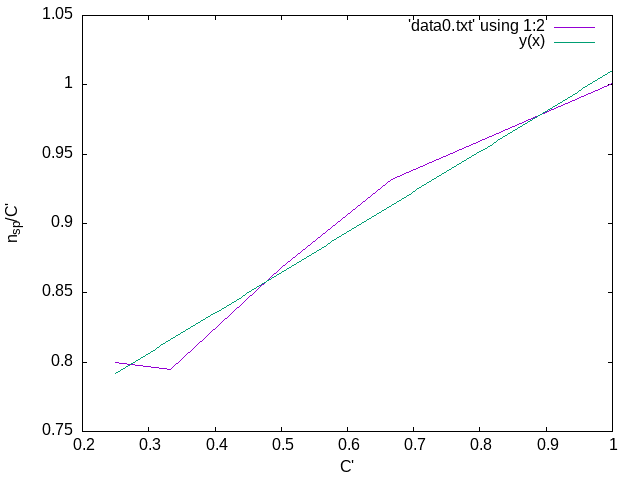
\includegraphics[width=.9\linewidth]{../data/out0.png}
\end{center}
\begin{verbatim}
iter      chisq       delta/lim  lambda   k             b            
   0 2.4294759800e+00   0.00e+00  8.29e-01    1.000000e+00   1.000000e+00
   1 5.2924403774e-02  -4.49e+06  8.29e-02    6.124020e-01   5.976467e-01
   2 9.8153532530e-04  -5.29e+06  8.29e-03    2.984907e-01   7.148691e-01
   3 9.6241239274e-04  -1.99e+03  8.29e-04    2.911840e-01   7.190487e-01
   4 9.6241239150e-04  -1.29e-04  8.29e-05    2.911821e-01   7.190498e-01
iter      chisq       delta/lim  lambda   k             b            

After 4 iterations the fit converged.
final sum of squares of residuals : 0.000962412
rel. change during last iteration : -1.28893e-09

degrees of freedom    (FIT_NDF)                        : 3
rms of residuals      (FIT_STDFIT) = sqrt(WSSR/ndf)    : 0.017911
variance of residuals (reduced chisquare) = WSSR/ndf   : 0.000320804

Final set of parameters            Asymptotic Standard Error
=======================            ==========================
k               = 0.291182         +/- 0.03004      (10.32%)
b               = 0.71905          +/- 0.01836      (2.553%)

correlation matrix of the fit parameters:
#                  k      b      
k               1.000 
b              -0.900  1.000 

\end{verbatim}
拟合出的曲线如下:
\[
\frac{\eta_{sp}}{C'}=0.2912C'+0.7191
\]

由关系式:
\[
\frac{\eta_{sp}}{C'}=[\eta]C_{0}+k[\eta]^{2}C_{0}^{2}C'
\]
有特性粘数:
\[
[\eta]=\frac{A}{C_{0}}=\frac{0.7191}{0.02011}=35.76mL/g
\]
将得到的[\(\eta\)]代入到[\(\eta\)]=KM\textsuperscript{a},粘均分子量:
\[
\bar{M_{\eta}}=\left(\frac{[\eta]}{K}\right)^{\frac{1}{a}}
\]
从 Polymer Handbook 查到:聚乙二醇-水溶液,在 30°C时, K=0.0125mL/g,
a=0.78 。

因此:
\[
\bar{M_{\eta}}=(35.76/0.0125)^{\frac{1}{0.78}}=27001.89
\]


\item 
\label{sec:org18f8919}
\[
ln\eta_{r}/C' \sim C'
\]
\begin{center}
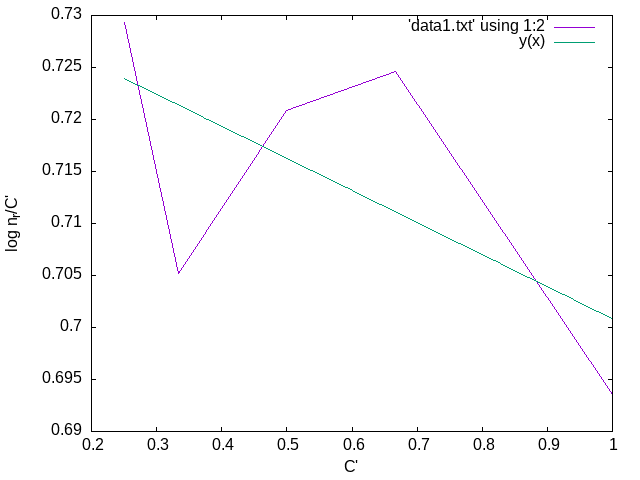
\includegraphics[width=.9\linewidth]{../data/out1.png}
\end{center}
\begin{verbatim}
iter      chisq       delta/lim  lambda   k             b            
   0 1.7269093784e-01   0.00e+00  5.24e-01    2.911821e-01   7.190498e-01
   1 2.9297365522e-02  -4.89e+05  5.24e-02    2.489217e-01   5.913640e-01
   2 7.5646011188e-04  -3.77e+06  5.24e-03   -6.563501e-03   7.181953e-01
   3 5.4656762518e-04  -3.84e+04  5.24e-04   -3.083087e-02   7.316768e-01
   4 5.4656743385e-04  -3.50e-02  5.24e-05   -3.085406e-02   7.316897e-01
iter      chisq       delta/lim  lambda   k             b            

After 4 iterations the fit converged.
final sum of squares of residuals : 0.000546567
rel. change during last iteration : -3.50053e-07

degrees of freedom    (FIT_NDF)                        : 3
rms of residuals      (FIT_STDFIT) = sqrt(WSSR/ndf)    : 0.0134977
variance of residuals (reduced chisquare) = WSSR/ndf   : 0.000182189

Final set of parameters            Asymptotic Standard Error
=======================            ==========================
k               = -0.0308541       +/- 0.02264      (73.36%)
b               = 0.73169          +/- 0.01384      (1.891%)

correlation matrix of the fit parameters:
#                k      b      
k               1.000 
b              -0.900  1.000 

\end{verbatim}
拟合出的曲线如下:
\[
\frac{ln\eta_{r}}{C'}=-0.03085C'+0.7317
\]

由关系式:
\[
\frac{ln\eta_{r}}{C'}=[\eta]C_{0}-\beta[\eta]^{2}C_{0}^{2}C'
\]
有特性粘数:
\[
[\eta]=\frac{A}{C_{0}}=\frac{0.7317}{0.02011}=36.38mL/g
\]
将得到的[\(\eta\)]代入到[\(\eta\)]=KM\textsuperscript{a},粘均分子量:
\[
\bar{M_{\eta}}=\left(\frac{[\eta]}{K}\right)^{\frac{1}{a}}
\]
从 Polymer Handbook 查到:聚乙二醇-水溶液,在 30°C时, K=0.0125mL/g,
a=0.78 。

因此:
\[
\bar{M_{\eta}}=(36.38/0.0125)^{\frac{1}{0.78}}=27603.55
\]
\end{enumerate}


\section{利用外推得到浓度为0的时间为t\textsubscript{0}计算粘均分子量}
\label{sec:orgf1f4f69}
以 t 对 C'作图,结果如下:

\[
t\sim C'
\]

\begin{center}
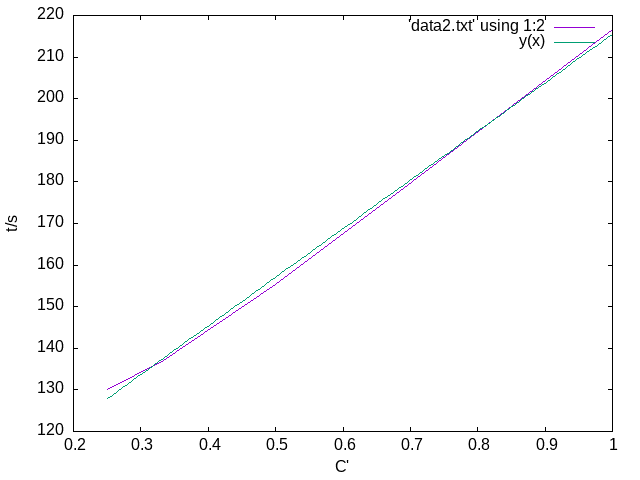
\includegraphics[width=.9\linewidth]{../data/out2.png}
\end{center}
\begin{verbatim}
iter      chisq       delta/lim  lambda   k             b            
   0 1.3642203690e+05   0.00e+00  5.18e-01   -3.085406e-02   7.316897e-01
   1 5.9314533614e+03  -2.20e+06  5.18e-02    2.605624e-01   1.480364e+02
   2 3.8206228066e+03  -5.52e+04  5.18e-03    1.334931e+01   1.555703e+02
   3 3.0933321663e+01  -1.23e+07  5.18e-04    1.092705e+02   1.028217e+02
   4 1.0424688989e+01  -1.97e+05  5.18e-05    1.168591e+02   9.864752e+01
   5 1.0424676153e+01  -1.23e-01  5.18e-06    1.168651e+02   9.864421e+01
iter      chisq       delta/lim  lambda   k             b            

After 5 iterations the fit converged.
final sum of squares of residuals : 10.4247
rel. change during last iteration : -1.23129e-06

degrees of freedom    (FIT_NDF)                        : 3
rms of residuals      (FIT_STDFIT) = sqrt(WSSR/ndf)    : 1.86411
variance of residuals (reduced chisquare) = WSSR/ndf   : 3.47489

Final set of parameters            Asymptotic Standard Error
=======================            ==========================
k               = 116.865          +/- 3.126        (2.675%)
b               = 98.6442          +/- 1.911        (1.937%)

correlation matrix of the fit parameters:
#                k      b      
k               1.000 
b              -0.900  1.000 

\end{verbatim}
拟合出的曲线如下:
\[
t=116.87C'+98.64
\]
外推浓度为 0 时有
\[
t_{0}^{\*}=98.64
\]
由:
\[
\eta_{r}=\frac{\eta}{\eta_{0}}\approx \frac{t}{t_{0}}
\]
和
\[
\eta_{sp}=\eta_{r}-1\approx \frac{t}{t_{0}}-1
\]
重新计算出相对粘度和增比粘度,结果列于下表中:
\begin{center}
\begin{tabular}{rlrrrrr}
加入溶剂量(ml) & 相对浓度(C') & 平均流出时间 & \(\eta\)\textsubscript{r} & \(\eta\)\textsubscript{sp} & \(\eta\)\textsubscript{sp}/C' & ln\(\eta\)\textsubscript{r}/C'\\
\hline
0 & 1 & 216.7 & 2.197 & 1.197 & 1.197 & 0.7871\\
5 & 2/3 & 175.6 & 1.780 & 0.780 & 1.170 & 0.8649\\
5 & 1/2 & 155.3 & 1.574 & 0.574 & 1.148 & 0.9072\\
10 & 1/3 & 137.0 & 1.389 & 0.389 & 1.167 & 0.9858\\
10 & 1/4 & 130.0 & 1.318 & 0.318 & 1.272 & 1.1045\\
\end{tabular}
\end{center}

以\(\eta_{sp}/C'\) , 和\(ln\eta_{r}/C'\) , 分别对C'作图, 结果如下:

\begin{enumerate}
\item 
\label{sec:org92b1bd0}
\[
\eta_{sp}/C'\sim C'
\]
\begin{center}
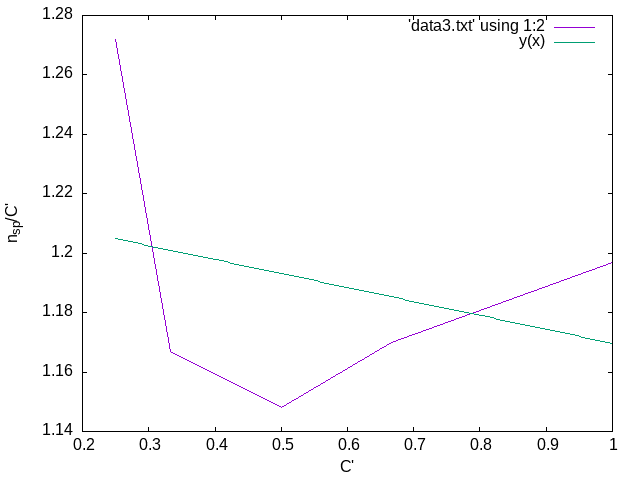
\includegraphics[width=.9\linewidth]{../data/out3.png}
\end{center}
\begin{verbatim}
iter      chisq       delta/lim  lambda   k             b            
   0 3.8851664275e-01   0.00e+00  8.22e-01   -3.802376e-01   1.139031e+00
   1 4.2687573123e-02  -8.10e+05  8.22e-02   -3.442369e-01   1.357386e+00
   2 9.1240488669e-03  -3.68e+05  8.22e-03   -8.236129e-02   1.236225e+00
   3 8.6784811143e-03  -5.13e+03  8.22e-04   -4.701357e-02   1.216658e+00
   4 8.6784802936e-03  -9.46e-03  8.22e-05   -4.696553e-02   1.216631e+00
iter      chisq       delta/lim  lambda   k             b            

After 4 iterations the fit converged.
final sum of squares of residuals : 0.00867848
rel. change during last iteration : -9.45647e-08

degrees of freedom    (FIT_NDF)                        : 3
rms of residuals      (FIT_STDFIT) = sqrt(WSSR/ndf)    : 0.053785
variance of residuals (reduced chisquare) = WSSR/ndf   : 0.00289283

Final set of parameters            Asymptotic Standard Error
=======================            ==========================
k               = -0.0469655       +/- 0.0902       (192.1%)
b               = 1.21663          +/- 0.05513      (4.532%)

correlation matrix of the fit parameters:
#                k      b      
k               1.000 
b              -0.900  1.000 

\end{verbatim}
拟合出的曲线如下:
\[
\frac{\eta_{sp}}{C'}=-0.04697C'+1.2166
\]

由关系式:
\[
\frac{\eta_{sp}}{C'}=[\eta]C_{0}+k[\eta]^{2}C_{0}^{2}C'
\]
有特性粘数:
\[
[\eta]=\frac{A}{C_{0}}=\frac{1.2166}{0.02011}=60.50mL/g
\]
将得到的[\(\eta\)]代入到[\(\eta\)]=KM\textsuperscript{a},粘均分子量:
\[
\bar{M_{\eta}}=\left(\frac{[\eta]}{K}\right)^{\frac{1}{a}}
\]
从 Polymer Handbook 查到:聚乙二醇-水溶液,在 30°C时, K=0.0125mL/g,
a=0.78 。

因此:
\[
\bar{M_{\eta}}=(60.50/0.0125)^{\frac{1}{0.78}}=52982.88
\]
\item 
\label{sec:org6eeb011}

\[
ln\eta_{r}/C' \sim C'
\]
\begin{center}
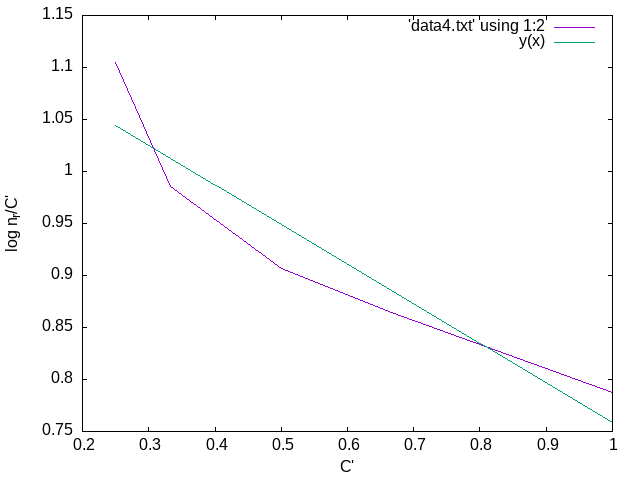
\includegraphics[width=.9\linewidth]{../data/out4.png}
\end{center}
\begin{verbatim}
iter      chisq       delta/lim  lambda   k             b            
   0 1.2654909855e+00   0.00e+00  5.12e-01    1.184775e+00  -2.630532e-05
   1 1.2423365770e+00  -1.86e+03  5.12e-02    1.286407e+00  -2.630239e-05
   2 1.2421430036e+00  -1.56e+01  5.12e-03    1.296559e+00  -2.601631e-05
   3 1.2420809816e+00  -4.99e+00  5.12e-04    1.296527e+00   2.590178e-06
   4 1.2359021711e+00  -5.00e+02  5.12e-05    1.292327e+00   2.856072e-03
   5 7.9217456306e-01  -5.60e+04  5.12e-06    9.565859e-01   2.309251e-01
   6 8.4832707736e-03  -9.24e+06  5.12e-07   -3.290473e-01   1.104257e+00
   7 7.3324487462e-03  -1.57e+04  5.12e-08   -3.802172e-01   1.139017e+00
   8 7.3324485638e-03  -2.49e-03  5.12e-09   -3.802376e-01   1.139031e+00
iter      chisq       delta/lim  lambda   k             b            

After 8 iterations the fit converged.
final sum of squares of residuals : 0.00733245
rel. change during last iteration : -2.4863e-08

degrees of freedom    (FIT_NDF)                        : 3
rms of residuals      (FIT_STDFIT) = sqrt(WSSR/ndf)    : 0.0494383
variance of residuals (reduced chisquare) = WSSR/ndf   : 0.00244415

Final set of parameters            Asymptotic Standard Error
=======================            ==========================
k               = -0.380238        +/- 0.08291      (21.8%)
b               = 1.13903          +/- 0.05068      (4.449%)

correlation matrix of the fit parameters:
#                k      b      
k               1.000 
b              -0.900  1.000 

\end{verbatim}
拟合出的曲线如下:
\[
\frac{ln\eta_{r}}{C'}=-0.3802C'+1.1390
\]

由关系式:
\[
\frac{ln\eta_{r}}{C'}=[\eta]C_{0}-\beta[\eta]^{2}C_{0}^{2}C'
\]
有特性粘数:
\[
[\eta]=\frac{A}{C_{0}}=\frac{1.1390}{0.02011}=56.64mL/g
\]
将得到的[\(\eta\)]代入到[\(\eta\)]=KM\textsuperscript{a},粘均分子量:
\[
\bar{M_{\eta}}=\left(\frac{[\eta]}{K}\right)^{\frac{1}{a}}
\]
从 Polymer Handbook 查到:聚乙二醇-水溶液,在 30°C时, K=0.0125mL/g,
a=0.78 。

因此:
\[
\bar{M_{\eta}}=(56.64/0.0125)^{\frac{1}{0.78}}=48689.80
\]
\end{enumerate}
\end{document}
